\documentclass{article}
\usepackage{amsthm}
\usepackage{amssymb}
\usepackage{pgf, tikz}
\usetikzlibrary{arrows, automata}
\begin{document}
\title{Homework 12}
\author{Will Boland}
\maketitle

\textbf{Question 1}\newline
A) $\forall$x$\exists$y((E(y) $\wedge$ T(x)) $\rightarrow$ R(x, y))\newline
B) $\neg$$\exists$x$\forall$y(T(y) $\rightarrow$ R(x, y))\newline
C) $\forall$x(E(x) $\rightarrow$ $\neg$$\exists$y(T(y)$\wedge$R(x, y)))\newline
D) $\exists$x$\forall$y(E(y) $\rightarrow$ $\neg$R(x, y))\newline
E) All textbooks are referenced by a book.\newline
F) NOTE: T(x) was supposed to be T(y): There is a book that does not reference any textbook.\newline
G) All textbooks have a book that they don't reference\newline\newline

\textbf{Question 2}\newline
A) \newline
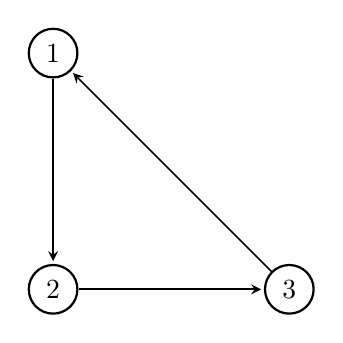
\begin{tikzpicture}[
            > = stealth, % arrow head style
            shorten > = 1pt, % don't touch arrow head to node
            auto,
            node distance = 3cm, % distance between nodes
            semithick % line style
        ]

        \tikzstyle{every state}=[
            draw = black,
            thick,
            fill = white,
            minimum size = 4mm
        ]

	\node[state] (1) {$1$};
	\node[state] (2) [below of=1] {$2$};
	\node[state] (3) [right of=2] {$3$};
	
        \path[->] (1) edge node {} (2);
        \path[->] (2) edge node {} (3);
        \path[->] (3) edge node {} (1);

    \end{tikzpicture}
\newline\newline
B)	All integers point to at least one real number\newline
	All integers, there exists a real number that is not pointed to by an integer.\newline
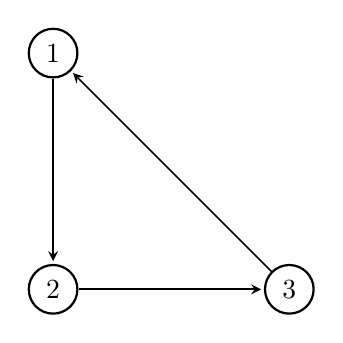
\begin{tikzpicture}[
            > = stealth, % arrow head style
            shorten > = 1pt, % don't touch arrow head to node
            auto,
            node distance = 3cm, % distance between nodes
            semithick % line style
        ]

        \tikzstyle{every state}=[
            draw = black,
            thick,
            fill = white,
            minimum size = 4mm
        ]

	\node[state] (1) {$1$};
	\node[state] (2) [below of=1] {$2$};
	\node[state] (3) [right of=2] {$3$};
	
        \path[->] (1) edge node {} (2);
        \path[->] (2) edge node {} (3);
        \path[->] (3) edge node {} (1);

    \end{tikzpicture}
\newline\newline
C) All real numbers point to a negative number.\newline
There does not exist a real number that points to all negative numbers.\newline
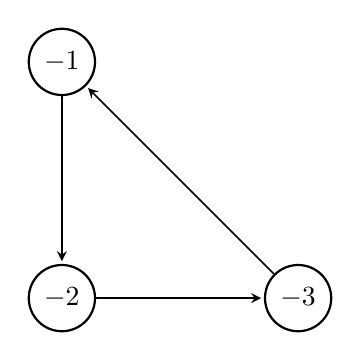
\begin{tikzpicture}[
            > = stealth, % arrow head style
            shorten > = 1pt, % don't touch arrow head to node
            auto,
            node distance = 3cm, % distance between nodes
            semithick % line style
        ]

        \tikzstyle{every state}=[
            draw = black,
            thick,
            fill = white,
            minimum size = 4mm
        ]

	\node[state] (1) {$-1$};
	\node[state] (2) [below of=1] {$-2$};
	\node[state] (3) [right of=2] {$-3$};
	
        \path[->] (1) edge node {} (2);
        \path[->] (2) edge node {} (3);
        \path[->] (3) edge node {} (1);

    \end{tikzpicture}
\newline\newline\newline

\textbf{Question 3}\newline
Example: L = \{("lol", "lol"), ("hello", "hi"), ("hi", "hello"), ("lol, "hi")\}\newline\newline

\textbf{Question 4}\newline
\textbf{Claim: } For any sets A, B, C, D, and E, if D$\cap$B$\subseteq$A$\setminus$C, then D$\cap$E$\subseteq$E$\setminus$(B$\cap$C)\newline\newline
\textit{Proof}\newline
Choose sets A, B, C, D, and E and assume Assume D$\cap$B$\subseteq$A$\setminus$C\newline
|	Choose D $\cap$ E\newline
|	So, x$\in$D and x$\in$E\newline
|	From x$\in$D$\cap$B, x$\in$D and x$\in$B\newline
|	From D$\cap$B$\subseteq$A$\setminus$C, so x$\in$A but x$\notin$C\newline
|	So, because x$\in$B and x$\notin$C and x$\in$E, E$\setminus$(B$\cap$C)\newline
Therefore, if D$\cap$B$\subseteq$A$\setminus$, then D$\cap$E$\subseteq$(B$\cap$C)$\square$\newline\newline

\textbf{Question 5}\newline
\textbf{Claim: } The cube of an odd \# is odd\newline\newline
\textit{Proof}\newline
Choose an odd number x\newline
So there exists an integer k with x = 2k + 1. (Side note: In class he said this would get half credit if stopped right here)\newline
${x^3 = (2k+1)^3}$\newline
= (2k+1)(2k+1)(2k+1)\newline
= ${(4k^2 + 4k + 1)(2k+1)}$\newline
= ${8k^3 + 12k^2 + 6k + 1}$\newline
= ${2(4k^3 + 6k^2 + 3k) + 1}$\newline
Since 4, k, 6, and 3 are integers, so is ${4k^3 + 6k^2 + 3k}$\newline
Therefore ${x^3}$ is odd $\square$\newline\newline

\textbf{Question 6}\newline
\textbf{Claim: } Prove R is transitive\newline\newline

\textit{Proof}\newline
Choose real numbers x, y, and z and assume R(x, y) and R(y, z)\newline
So ${x-y>1}$ and ${y-z>1}$ (Side note: In class he said this would get half credit if stopped right here)\newline
${(x-y)+(y-z) > 1 + 1}$\newline
${x-z > 2}$\newline
${> 1}$\newline
So ${x-z>1}$ $\square$\newline\newline


\enddocument
















